\documentclass{article}
\usepackage{amsmath,amssymb,amsthm,graphicx,setspace,fullpage,verbatim,listings,xcolor}

\onehalfspace

\title{\bf\huge AI+X: Report 2}
\author{Hanxi Lin}

\lstset{
	backgroundcolor=\color{gray!10},   % 背景色
	basicstyle=\ttfamily\footnotesize, % 基本字体样式
	breaklines=true,                  % 自动换行
	frame=noframe,                     % 边框样式
	numbers=left,                     % 行号位置
	numberstyle=\tiny\color{gray},    % 行号样式
	keywordstyle=\color{blue},        % 关键字样式
	commentstyle=\color{green!50!black}, % 注释样式
	stringstyle=\color{orange},       % 字符串样式
	showstringspaces=false            % 不显示字符串中的空格
}

\begin{document}
\maketitle

\begin{figure}[h]
    \centering
    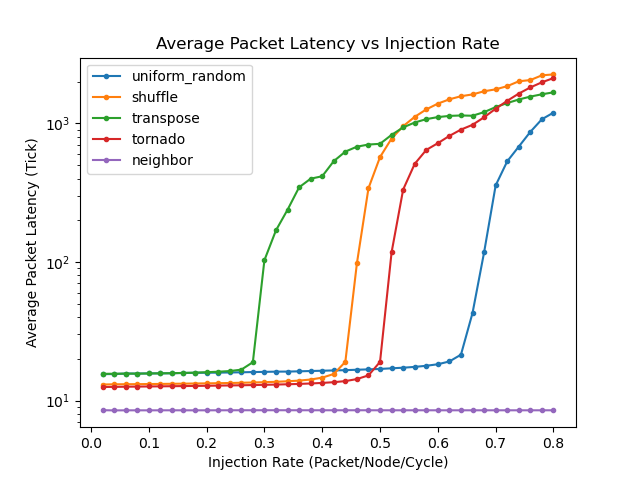
\includegraphics[width=0.49\textwidth]{lab2-SYNTHETIC_TRAFFIC.png}
    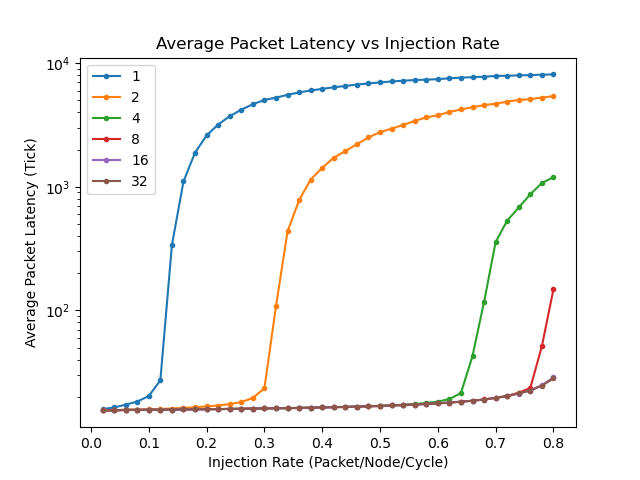
\includegraphics[width=0.49\textwidth]{lab2-VCS_PER_VNET.png}
    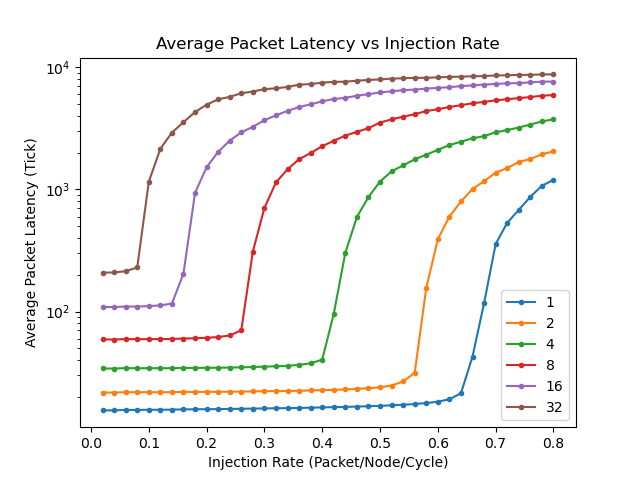
\includegraphics[width=0.49\textwidth]{lab2-ROUTER_LATENCY.png}
    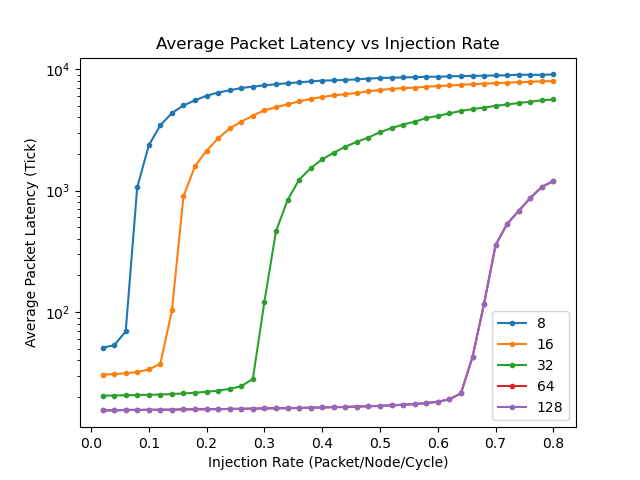
\includegraphics[width=0.49\textwidth]{lab2-LINK_WIDTH_BITS.png}
    \caption{Average Packet Latency vs. Injection Rate under different configurations}
\end{figure}

\section*{Task 1\&2}
By running the shell script in appendix, we generated the four figures above. Here we generated the latency-injection rate curve instead of the latency-throughput curve, since we can still clearly observe the congestion point, and we can better analyse the behavior after congestion.

\begin{itemize}
    \item \textbf{SYNTHETIC TRAFFIC}: As figure 1 shows, when the injection rate is low, the average packet latency is dominated by the network latency, which is highly correlated to the average hops, where
    $$H_{uniform}\approx 5.23,H_{transpose}\approx 5.27,H_{shuffle}\approx 4.01,H_{tornado}\approx 3.74,H_{neighbor}\approx 1.75$$
	Whose order is identical as the order of average packet latency at low load. As the injection rate increases, the network becomes congested, and the average packet latency increases dramatically. The structure of transpose traffic makes the traffic concentrate on the diagonal and has the lowest congestion point, while uniform random traffic splits the traffic evenly and has the highest congestion point. After congestion, the average packet latency is dominated by the queuing latency, which is highly correlated to the injection rate. The order of average packet latency after congestion is identical as the order of injection rate at congestion point. 
    \item \textbf{VCS PER VNET}: As figure 2 shows, when the injection rate is low, the average packet latency is almost identical under different VCs per VNet, since the network latency dominates. As the injection rate increases, the network becomes congested, and the average packet latency increases dramatically. More VCs per VNet can alleviate the congestion and increase the congestion point. After congestion, the average packet latency is dominated by the queuing latency, which is highly correlated to the injection rate. The order of average packet latency after congestion is identical as the order of injection rate at congestion point.
    \item \textbf{ROUTER LATENCY}: As figure 3 shows, when the injection rate is low, the average packet latency is dominated by the network latency, which is highly correlated to the router latency.
    \item \textbf{LINK WIDTH BITS}: As figure 4 shows, link width bits decides the number of cycles neccessary to transmit a flit. So the network latency and congestion point is almost linearly correlated to the link width bits. When the link width bits is large enough, a flit only need one hop to transmit, the latency no longer keep decreasing.
\end{itemize}

\section*{Task 3}
\begin{enumerate}
	\item Transmission, propagation, processing, and queuing delay. In NoC we needn't consider the propagation delay since the distance is very short. The processing delay is also very small compared to the transmission and queuing delay. When the network is not congested, the transmission delay dominates the total delay. When the network is congested, the queuing delay dominates the total delay.
	\item 4 flits and virtual channel flow control.
\end{enumerate}


\section*{Appendix}
\begin{lstlisting}[language=bash]
#! /bin/bash

NUM_CPUS=64
SIM_CYCLES=10000

echo > network_stats.txt

for SYNTH in uniform_random shuffle transpose tornado neighbor
do
	echo "SYNTHETIC TRAFFIC: $SYNTH" >> network_stats.txt
	for INJ_RATE in 0.02 0.04 0.06 0.08 0.10 0.12 0.14 0.16 0.18 0.20 0.22 0.24 0.26 0.28 0.30 0.32 0.34 0.36 0.38 0.40 0.42 0.44 0.46 0.48 0.50 0.52 0.54 0.56 0.58 0.60 0.62 0.64 0.66 0.68 0.70 0.72 0.74 0.76 0.78 0.80
	do
		./build/NULL/gem5.opt \
		configs/example/garnet_synth_traffic.py \
		--network=garnet --num-cpus=$NUM_CPUS --num-dirs=64 \
		--topology=Mesh_XY --mesh-rows=8 \
		--inj-vnet=0 --synthetic=$SYNTH \
		--sim-cycles=$SIM_CYCLES --injectionrate=$INJ_RATE
		INJ_TOT=$(grep -Eo "packets_injected::total\s*[0-9.]*" m5out/stats.txt | grep -Eo "[0-9.]*")
		RECV_TOT=$(grep -Eo "packets_received::total\s*[0-9.]*" m5out/stats.txt | grep -Eo "[0-9.]*")
		RECV_RATE=$(echo "scale=6;$RECV_TOT/$NUM_CPUS/$SIM_CYCLES" | bc)
		AVG_PKT_QUEUE_LATENCY=$(grep -Eo "average_packet_queueing_latency\s*[0-9.]*" m5out/stats.txt | grep -Eo "[0-9.]*")
		AVG_PKT_NETWK_LATENCY=$(grep -Eo "average_packet_network_latency\s*[0-9.]*" m5out/stats.txt | grep -Eo "[0-9.]*")
		AVG_PKT_LATENCY=$(grep -Eo "average_packet_latency\s*[0-9.]*" m5out/stats.txt | grep -Eo "[0-9.]*")
		AVG_HOPS=$(grep -Eo "average_hops\s*[0-9.]*" m5out/stats.txt | grep -Eo "[0-9.]*")
		echo "[$INJ_RATE, $INJ_TOT, $RECV_TOT, $RECV_RATE, $AVG_PKT_QUEUE_LATENCY, $AVG_PKT_NETWK_LATENCY, $AVG_PKT_LATENCY, $AVG_HOPS]" >> network_stats.txt
	done
	echo >> network_stats.txt
done

python3 plot.py

echo > network_stats.txt

for VCS_PER_VNET in 1 2 4 8 16 32
do
	echo "VCS PER VNET: $VCS_PER_VNET" >> network_stats.txt
	for INJ_RATE in 0.02 0.04 0.06 0.08 0.10 0.12 0.14 0.16 0.18 0.20 0.22 0.24 0.26 0.28 0.30 0.32 0.34 0.36 0.38 0.40 0.42 0.44 0.46 0.48 0.50 0.52 0.54 0.56 0.58 0.60 0.62 0.64 0.66 0.68 0.70 0.72 0.74 0.76 0.78 0.80
	do
		./build/NULL/gem5.opt \
		configs/example/garnet_synth_traffic.py \
		--network=garnet --num-cpus=$NUM_CPUS --num-dirs=64 \
		--topology=Mesh_XY --mesh-rows=8 --vcs-per-vnet=$VCS_PER_VNET\
		--inj-vnet=0 --synthetic=uniform_random \
		--sim-cycles=$SIM_CYCLES --injectionrate=$INJ_RATE
		INJ_TOT=$(grep -Eo "packets_injected::total\s*[0-9.]*" m5out/stats.txt | grep -Eo "[0-9.]*")
		RECV_TOT=$(grep -Eo "packets_received::total\s*[0-9.]*" m5out/stats.txt | grep -Eo "[0-9.]*")
		RECV_RATE=$(echo "scale=6;$RECV_TOT/$NUM_CPUS/$SIM_CYCLES" | bc)
		AVG_PKT_QUEUE_LATENCY=$(grep -Eo "average_packet_queueing_latency\s*[0-9.]*" m5out/stats.txt | grep -Eo "[0-9.]*")
		AVG_PKT_NETWK_LATENCY=$(grep -Eo "average_packet_network_latency\s*[0-9.]*" m5out/stats.txt | grep -Eo "[0-9.]*")
		AVG_PKT_LATENCY=$(grep -Eo "average_packet_latency\s*[0-9.]*" m5out/stats.txt | grep -Eo "[0-9.]*")
		AVG_HOPS=$(grep -Eo "average_hops\s*[0-9.]*" m5out/stats.txt | grep -Eo "[0-9.]*")
		echo "[$INJ_RATE, $INJ_TOT, $RECV_TOT, $RECV_RATE, $AVG_PKT_QUEUE_LATENCY, $AVG_PKT_NETWK_LATENCY, $AVG_PKT_LATENCY, $AVG_HOPS]" >> network_stats.txt
	done
	echo >> network_stats.txt
done

python3 plot.py

echo > network_stats.txt

for ROUTER_LATENCY in 1 2 4 8 16 32
do
	echo "ROUTER LATENCY: $ROUTER_LATENCY" >> network_stats.txt
	for INJ_RATE in 0.02 0.04 0.06 0.08 0.10 0.12 0.14 0.16 0.18 0.20 0.22 0.24 0.26 0.28 0.30 0.32 0.34 0.36 0.38 0.40 0.42 0.44 0.46 0.48 0.50 0.52 0.54 0.56 0.58 0.60 0.62 0.64 0.66 0.68 0.70 0.72 0.74 0.76 0.78 0.80
	do
		./build/NULL/gem5.opt \
		configs/example/garnet_synth_traffic.py \
		--network=garnet --num-cpus=$NUM_CPUS --num-dirs=64 \
		--topology=Mesh_XY --mesh-rows=8 --router-latency=$ROUTER_LATENCY\
		--inj-vnet=0 --synthetic=uniform_random \
		--sim-cycles=$SIM_CYCLES --injectionrate=$INJ_RATE
		INJ_TOT=$(grep -Eo "packets_injected::total\s*[0-9.]*" m5out/stats.txt | grep -Eo "[0-9.]*")
		RECV_TOT=$(grep -Eo "packets_received::total\s*[0-9.]*" m5out/stats.txt | grep -Eo "[0-9.]*")
		RECV_RATE=$(echo "scale=6;$RECV_TOT/$NUM_CPUS/$SIM_CYCLES" | bc)
		AVG_PKT_QUEUE_LATENCY=$(grep -Eo "average_packet_queueing_latency\s*[0-9.]*" m5out/stats.txt | grep -Eo "[0-9.]*")
		AVG_PKT_NETWK_LATENCY=$(grep -Eo "average_packet_network_latency\s*[0-9.]*" m5out/stats.txt | grep -Eo "[0-9.]*")
		AVG_PKT_LATENCY=$(grep -Eo "average_packet_latency\s*[0-9.]*" m5out/stats.txt | grep -Eo "[0-9.]*")
		AVG_HOPS=$(grep -Eo "average_hops\s*[0-9.]*" m5out/stats.txt | grep -Eo "[0-9.]*")
		echo "[$INJ_RATE, $INJ_TOT, $RECV_TOT, $RECV_RATE, $AVG_PKT_QUEUE_LATENCY, $AVG_PKT_NETWK_LATENCY, $AVG_PKT_LATENCY, $AVG_HOPS]" >> network_stats.txt
	done
	echo >> network_stats.txt
done

python3 plot.py

echo > network_stats.txt

for LINK_WIDTH_BITS in 8 16 32 64 128
do
	echo "LINK WIDTH BITS: $LINK_WIDTH_BITS" >> network_stats.txt
	for INJ_RATE in 0.02 0.04 0.06 0.08 0.10 0.12 0.14 0.16 0.18 0.20 0.22 0.24 0.26 0.28 0.30 0.32 0.34 0.36 0.38 0.40 0.42 0.44 0.46 0.48 0.50 0.52 0.54 0.56 0.58 0.60 0.62 0.64 0.66 0.68 0.70 0.72 0.74 0.76 0.78 0.80
	do
		./build/NULL/gem5.opt \
		configs/example/garnet_synth_traffic.py \
		--network=garnet --num-cpus=$NUM_CPUS --num-dirs=64 \
		--topology=Mesh_XY --mesh-rows=8 --link-width-bits=$LINK_WIDTH_BITS\
		--inj-vnet=0 --synthetic=uniform_random \
		--sim-cycles=$SIM_CYCLES --injectionrate=$INJ_RATE
		INJ_TOT=$(grep -Eo "packets_injected::total\s*[0-9.]*" m5out/stats.txt | grep -Eo "[0-9.]*")
		RECV_TOT=$(grep -Eo "packets_received::total\s*[0-9.]*" m5out/stats.txt | grep -Eo "[0-9.]*")
		RECV_RATE=$(echo "scale=6;$RECV_TOT/$NUM_CPUS/$SIM_CYCLES" | bc)
		AVG_PKT_QUEUE_LATENCY=$(grep -Eo "average_packet_queueing_latency\s*[0-9.]*" m5out/stats.txt | grep -Eo "[0-9.]*")
		AVG_PKT_NETWK_LATENCY=$(grep -Eo "average_packet_network_latency\s*[0-9.]*" m5out/stats.txt | grep -Eo "[0-9.]*")
		AVG_PKT_LATENCY=$(grep -Eo "average_packet_latency\s*[0-9.]*" m5out/stats.txt | grep -Eo "[0-9.]*")
		AVG_HOPS=$(grep -Eo "average_hops\s*[0-9.]*" m5out/stats.txt | grep -Eo "[0-9.]*")
		echo "[$INJ_RATE, $INJ_TOT, $RECV_TOT, $RECV_RATE, $AVG_PKT_QUEUE_LATENCY, $AVG_PKT_NETWK_LATENCY, $AVG_PKT_LATENCY, $AVG_HOPS]" >> network_stats.txt
	done
	echo >> network_stats.txt
done

python3 plot.py
\end{lstlisting}

\end{document}
